\section{Formule di quadratura numerica (approssimazione di integrali definiti)}
\footnote{Slide 10 PDF 25, 26-27, PG 105-114.}
Il problema da risolvere è quello di approssimare il valore dell'integrale nella forma
\begin{equation}\label{eq:probQuadratura}
    I(f)=\int_{a}^{b}f(x) dx,\quad -\infty<\overset{\footnotemark}{\boldsymbol{a<b}}<\infty ,
\end{equation}
dove $f:[a,b]\rightarrow\mathbb R$, almeno continua. In questa trattazione di approssimazione di integrali definiti è considerato solo il caso in cui $f$ è continua, per evitare singolarità integrabili nell'intervallo $[a,b]$ e non sarà considerato il caso di integrali definiti su insiemi illimitati. I metodi di approssimazione trattati saranno definiti mediante l'integrale di una approssimazione polinomiale a tratti di $f(x)$, in quanto l'integrale di un polinomio può essere calcolato facilmente ed in modo esatto.
\footnotetext{Se $a>b$ allora è applicato Riemann, $a$ e $b$ sono invertiti di segno. Se non è conosciuta la derivata prima di $f$, l'integrale è calcolato in forma chiusa. Spesso è necessario fornire un metodo numerico in questo intervallo. Questi metodi si chiamano "Forma di quadratura" (i quali consentono di determinare l'integrale esatto di una approssimazione della funzione $f$, per la quale è possibile l'integrazione). Prima è necessario studiare il condizionamento del problema dell'integrazione.}

Prima di trattare i metodi di approssimazione è studiato il condizionamento del problema, in cui la perturbazione è sulla funzione integranda $f(x)$. Studiare il condizionamento significa stabilire se al posto di $f$ è presente una sua perturbazione, ovvero quando il risultato è perturbato.

\begin{definition}[Numero di condizionamento]
    Supposta $\Tilde{f}(x)\in C^{(0)}[a,b]$, ovvero una perturbazione di $f(x)$, allora (vedi (\ref{eq:defNormaInfG})):
    \begin{equation*}
        \begin{matrix}
            \overbrace{\boldsymbol{|I(f)-I(\Tilde{f})|}}^{\footnotemark} &=& \left|\int_{a}^{b}f(x)dx-\int_{a}^{b}\Tilde{f}(x)dx\right| &=& \left|\int_{a}^{b}(f(x)-\Tilde{f}(x))dx\right|\\
             &\underset{\footnotemark}{\leq}&\int_{a}^{b}|f(x)-\Tilde{f}(x)|dx&\leq& ||f-\Tilde{f}||\cdot\int_{a}^{b}dx &=&\boldsymbol{(b-a)\cdot}\boldsymbol{||f-\Tilde{f}||},
        \end{matrix}
    \end{equation*}
    
    \addtocounter{footnote}{-1}
    \footnotetext{Errore del risultato.}
    
    \stepcounter{footnote}
    \footnotetext{Il valore assoluto di un integrale di una funzione è minore uguale dell'integrazione del valore assoluto della funzione. Questo è specificato anche dal criterio di integrabilità.}
    
    \noindent dove
    \begin{equation*}
        \boldsymbol{\kappa=(b-a)},\quad \boldsymbol{||f-\Tilde{f}||}=\underset{a\leq x\leq b}{\max} |f(x)-\Tilde{f}(x)|
    \end{equation*}
    definiscono, rispettivamente, il \textbf{numero di condizionamento del problema} (\ref{eq:probQuadratura}) e la misura l'\textbf{errore sui dati d'ingresso}.
\end{definition}

\subsection{Formule di Newton-Cotes}\label{ssec:formN-C}\footnote{Slide 10 PDF 25-26, PG 106-108.}
Le formule più semplici per l'approssimazione di $I(f)$ nell'intervallo $[a,b]$, dette \textbf{formule di Newton-Cotes}, sono ottenute calcolando l'integrale esatto del polinomio interpolante la funzione $f(x)$ su $n+1$ ascisse equidistanti, ovvero:
\begin{equation}\label{eq:condAscEqN-C}
    \begin{matrix}
        &x_i=a+ih,&\quad i=0,\hdots,n,\\
        &p_n(x_i)=f_i \equiv f(x_i),&\quad h=\frac{b-a}{n}.
    \end{matrix}
\end{equation}

Sia $p(x)$ il polinomio interpolante $f(x)$, è considerata la sua forma di Lagrange (\ref{eq:polLagrange})-(\ref{eq:formaKronecker}) per l'approssimazione di $I(f)$. Segue la definizione della \textbf{formula di Newton-Cotes di grado} $\boldsymbol n$ (esprimile in (\ref{eq:formN-C})):
\begin{equation*}
    I(f)\approx \int_a^b p(x)dx=\underbrace{\sum_{i=0}^n f_i\int_a^b L_{in}(x)dx}_{\footnotemark}\equiv I_n(f).
\end{equation*}\footnotetext{Questa è una formulazione ingombrante, cambiando intervallo è necessario ricalcolare gli $f_i$ (ovvero gli $f(x_i)$). Tramite la sommatoria è ottenuta una combinazione lineare dei valori della funzione $f$ pesata dagli integrali (i quali sono integrali del polinomio di Lagrange).}

Una formulazione più conveniente della precedente, poste le seguenti condizioni, per $x=a+th$ e $t\in [0,n]$:
\begin{enumerate}
    \item $\underbrace{x_i=a+ih}_{\footnotemark}\Rightarrow x_i\rightarrow i,\quad i=0,\hdots ,n$,
    \item $dx=\boldsymbol{h}dt\quad (h=\frac{b-a}{n}$, ovvero $h$ di (\ref{eq:condAscEqN-C})),
\end{enumerate}\footnotetext{Trasformazione lineare di $x=a+th$.}
è la seguente:
\begin{equation*}
    \begin{matrix}
        \int_a^b L_{in}(x)dx&=&h\int_0^nL_{in}(a+th)dt&\overset{x=a+th}{=}& h\int_0^n\prod_{j=0,j\neq i}^{n}\frac{\overbrace{(a+th)}^x-\overbrace{(a+jh)}^{x_j}}{\underbrace{(a+ih)}_{x_i}-\underbrace{(a+jh)}_{x_j}}dt\\
        &\overset{\footnotemark}{=}&h\underbrace{\int_0^n\prod_{j=0,j\neq i}^n\frac{t-j}{i-j}dt}_{c_{in}} &\equiv& \frac{b-a}{n}\, c_{in} &=& h\,c_{in}.
    \end{matrix}
\end{equation*}

\footnotetext{Semplificando $a$ e raggruppando $h$.}

Pertanto, la \textbf{formula di Newton-Cotes di grado} $\boldsymbol n$ è esprimibile come:
\begin{equation}\label{eq:formN-C}
    \boldsymbol{I_n(f)\approx h\sum_{i=0}^n f_ic_{in}},\quad \boldsymbol{c_{in}=\int_0^n\prod_{j=0, j\neq i}^n \frac{t-j}{i-j}dt.}
\end{equation}

Alcune proprietà dei coefficienti $\{c_{in}\}_{i\in\{0, \hdots,n\}}$ sono le seguenti:
\begin{enumerate}
    \item \footnotemark Dalla simmetria delle ascisse $\{x_i\}$ nell'intervallo $[a,b]$ segue che:
    \begin{equation}\label{eq:simmCoeffN-C}
        \boldsymbol{c_{in}=c_{n-i,n},\quad i=0,\hdots,n.}
    \end{equation}
    \footnotetext{Slide 13 PDF 25, PG 107. Questa proprietà deriva dal fatto che le ascisse di interpolazione sono simmetriche. Affinché la 1. valga è sufficiente che le ascisse siano simmetriche (non è richiesto che siano equidistanti).}
    \item \footnotemark \begin{equation}\label{eq:coeffN-CEq1}
        \boldsymbol{\frac{1}{n}\sum_{i=0}^{n}c_{in}=1}.
    \end{equation}
    \footnotetext{Slide 13 PDF 25, Teorema 5.1 PG 106.}
    \begin{proof}[Dimostrazione 2.]
        Se considerato $\boldsymbol{a=0},\, \boldsymbol{b=1}$ e $\boldsymbol{f(x)\equiv1}$ segue che, poiché $p(x)\equiv f(x)\equiv 1:$
        \begin{equation*}
            \int_0^1 1\cdot dx=1\equiv I_n(1)=\frac{1}{n}\sum_{i=0}^n1\cdot c_{in}=\frac{1}{n}\sum_{i=0}^nc_{in}.\quad\footnotemark
        \end{equation*}
        \footnotetext{Se $n=1$ sono presenti due coefficienti e non è necessario calcolarli perché è noto che siano uguali (la somma $c$ vale $\frac{1}{2}$). Se $n=2$ sono presenti tre coefficienti, è calcolato il primo (il quale è uguale all'ultimo) e l'altro è ottenuto tramite differenza tra il risultato e i due coefficienti uguali. Il calcolo dei coefficienti è spiegato tra poche righe.}
    \end{proof}
\end{enumerate}

Riassumendo: $I(f)\approx I(p_n)\equiv I_n(f)=\frac{b-a}{n}\sum_{i=0}^n f_i \int_0^n\prod_{j=0,j\neq i}^n\frac{t-j}{i-j}dt.$

\textbf{Utilizzando (\ref{eq:formN-C})-(\ref{eq:coeffN-CEq1}):}
\begin{enumerate}
    \item $\boldsymbol{\underline{n=1}}:\; c_{01},\, c_{11}$ sono i coefficienti (da calcolare, anche se non realmente) e dalle precedenti proprietà 1. e 2. segue che $c_{01}=c_{11}=\frac{1}{2}.$ Pertanto, quando il gardo è 1, \textbf{è definita la formula dei trapezi:}
    \begin{equation}\label{eq:formTrapezi}
        \boxed{\boldsymbol{I_1(f)=\frac{b-a}{2}(f(a)+f(b))},}
    \end{equation}
    la quale ha un importante significato geometrico, visibile in Figura \ref{fig:grafFormTrapezi}, ovvero quello di approssimare, nel caso di funzioni non negative, l'area sottesa dal grafico di $f(x)$ con quella del trapezio avente come vertici i punti $(a,0),(a,f(a)),(b,f(b)),(b,0)$.
    \item $\boldsymbol{\underline{n=2}}$: In questo caso sono presenti 3 coefficienti, ovvero $c_{02},\, c_{12}, \,c_{22},$ t.c.:
    \begin{enumerate}
        \item[P1:] $c_{02}+c_{12}+c_{22}=2$;
        \item[P2:] $c_{02}=c_{22}$ (per la sommatoria).
    \end{enumerate}
    Quindi è necessario calcolare un solo elemento, $c_{22}$, e non tre. È possibile calcolarlo come segue:
    \begin{equation*}
        \begin{matrix}
            \boldsymbol{c_{22}}&=&\int_0^2\frac{t}{2}\frac{t-1}{1}dt&=&\frac{1}{2}\int_0^2(t^2-t)dt&=&\\
            &&\frac{1}{2}\left[\frac{t^3}{3}-\frac{t^2}{2}\right]_0^2&=&\frac{1}{2}\left(\frac{8}{3}-2\right)&=&\boldsymbol{\frac{1}{3}}.
        \end{matrix}
    \end{equation*}
    Quindi $c_{02}=c_{22}=\frac{1}{3}\Rightarrow c_{12}=2-\frac{2}{3}=\frac{4}{3}$.
    La conseguenza di quanto scritto è la \textbf{formula di Simpson}, dato $x_0=a, x_2=b$ e $x_1=\frac{a+b}{2}$:
    \begin{equation}\label{eq:formSimpson}
        \boxed{\boldsymbol{I_2(f)=\frac{b-a}{6}\left(f(a)+4f\left(\frac{a+b}{2}\right)+f(b)\right)},}
    \end{equation}
\end{enumerate}

\begin{figure}
    \centering
    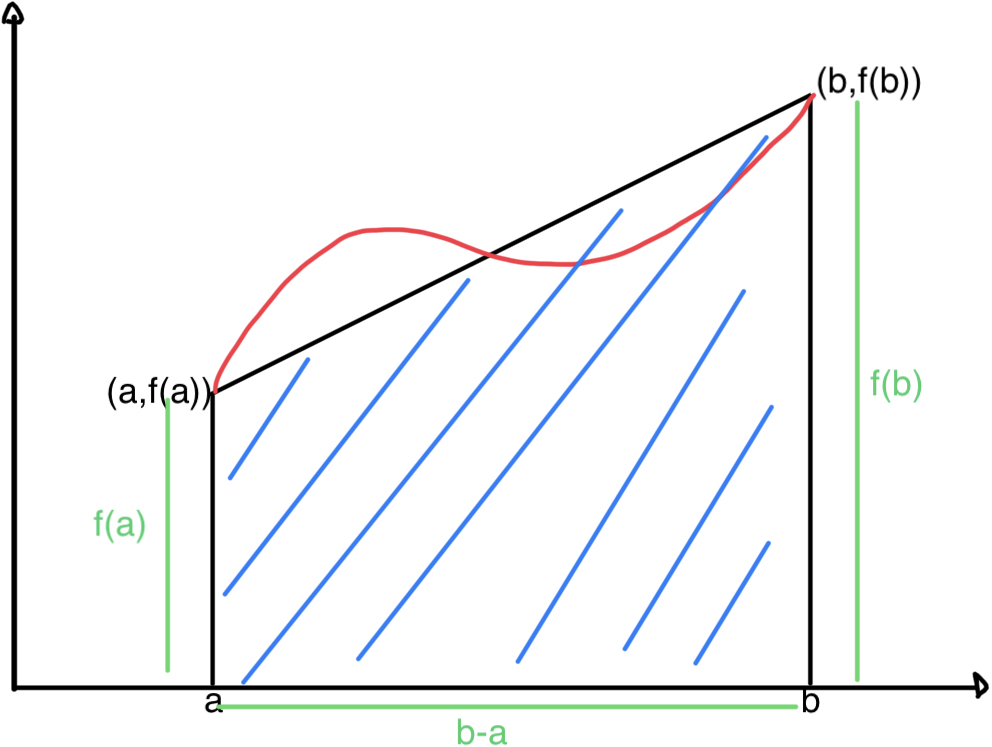
\includegraphics[width=0.5\textwidth]{immagini/grafFormTrapezi.png}
    \caption{Esempio del metodo dei trapezi ($f(a)$, $b-a$ ed $f(b)$ sono lunghezze).}\label{fig:grafFormTrapezi}
\end{figure}

\subsubsection{Condizionamento di una formula di Newton-Cotes}
\footnote{Slide 5-6 PDF 26, PG 108.}
Data una perturbazione $\Tilde{f}(x)$ di $f(x)$ e $c_{in}$, definita come in (\ref{eq:formN-C}), è possibile studiare come $\Tilde{f}(x)$ influisca su (\ref{eq:formTrapezi}), studiandone il condizionamento. In analogia con quanto visto per il condizionamento di (\ref{eq:probQuadratura}), è ottenuto quanto segue:

\begin{equation*}
    \begin{matrix}
        |I_n(f)-I_n(\Tilde{f})|&\overset{\footnotemark}{=}&\frac{b-a}{n}\left|\sum_{i=0}^n c_{in}f_i-\sum_{i=0}^n c_{in}\Tilde{f_i}\right|&=&\\
        \frac{b-a}{n}\left|\sum_{i=0}^n c_{in}\left(f_i-\Tilde{f_i}\right)\right|&\overset{\footnotemark}{\leq}&\frac{b-a}{n}\sum_{i=0}^n \left|c_{in}\left(f_i-\Tilde{f_i}\right)\right|&=&\\
        \frac{b-a}{n}\sum_{i=0}^n |c_{in}|\cdot\left|f_i-\Tilde{f_i}\right|&\leq&\left(\frac{b-a}{n}\sum_{i=0}^n|c_{in}|\right)\underset{i=0,\hdots,n}{\max}\left|f_i-\Tilde{f_i}\right|&\leq&\\
        && \underbrace{\left(\frac{b-a}{n}\sum_{i=0}^n|c_{in}|\right)}_{\boldsymbol{\kappa_n}}\cdot \equalto{\left|\left|f-\Tilde{f}\right|\right|}{\underset{a\leq x\leq b}{\max}||f(x)-\Tilde{f}(x)||}
    \end{matrix}
\end{equation*}
\addtocounter{footnote}{-1}
\footnotetext{Supposto di aver traspormato il problema in modo tale che $b>a$.}

\stepcounter{footnote}
\footnotetext{Diseguaglianza triangolare.}

\noindent dove $\boldsymbol{\kappa_n}$ è il \textbf{numero di condizionamento del problema} e $\boldsymbol{||f-\Tilde{f}||}$ misura l'\textbf{errore in ingresso}.

\begin{remark}
    \footnote{OSS Slide 6 PDF 26.} Se
    \begin{equation}\label{eq:coeffFormN-CGT0}
        \boldsymbol{\forall\, i=0,\hdots, n\; :\; c_{in}\leq 0,}
    \end{equation}
    allora:
    \begin{equation}\label{eq:nrCondN-C}
     \boldsymbol{\kappa_n}=\frac{b-a}{n}\sum_{i=0}^n|c_{in}|\overset{\footnotemark}{=}\frac{b-a}{\cancel{n}}\cancel{\sum_{i=0}^nc_{in}}\overset{\footnotemark}{=}b-a\boldsymbol{\equiv\kappa}.
    \end{equation}

\end{remark}
\addtocounter{footnote}{-1}
\footnotetext{Eliminato il modulo perché $c_{in}\geq 0$.}

\stepcounter{footnote}
\footnotetext{Per (\ref{eq:coeffN-CEq1}) ci sono le eliminazioni.}

Se i coefficienti della formula di Newton-Cotes sono non negativi allora il numero di condizionamento della formula di Newton-Cotes coincide con quello dell'integrale. Questo non significa che è ben condizionato: se l'integrale è ben condizionato allora lo è anche la funzione, se l'integrale è mal condizionato lo è anche la funzione. Ciò può essere riformulato affermando che \textbf{il mal condizionamento coincide con quello del problema continuo} (l'integrale $I(f)$).

Tuttavia, la proprietà (\ref{eq:coeffFormN-CGT0}) vale solo per $\boldsymbol{n=1,2,\hdots,7,9}$. Per tutti gli altri valori di $n$ compaiono pesi negativi ed il rapporto $\frac{\kappa_n}{\kappa}=\frac{1}{n}\sum_{i=0}^n|c_{in}|$ cresce molto rapidamente al crescere di $n$. Pertanto non è raccomandabile l'utilizzo di formule di Newton-Cotes di grado 8 o, genericamente, maggiori uguali a 10 (vedere Figura \ref{fig:knN-C}).

\begin{figure}[H]
    \centering
    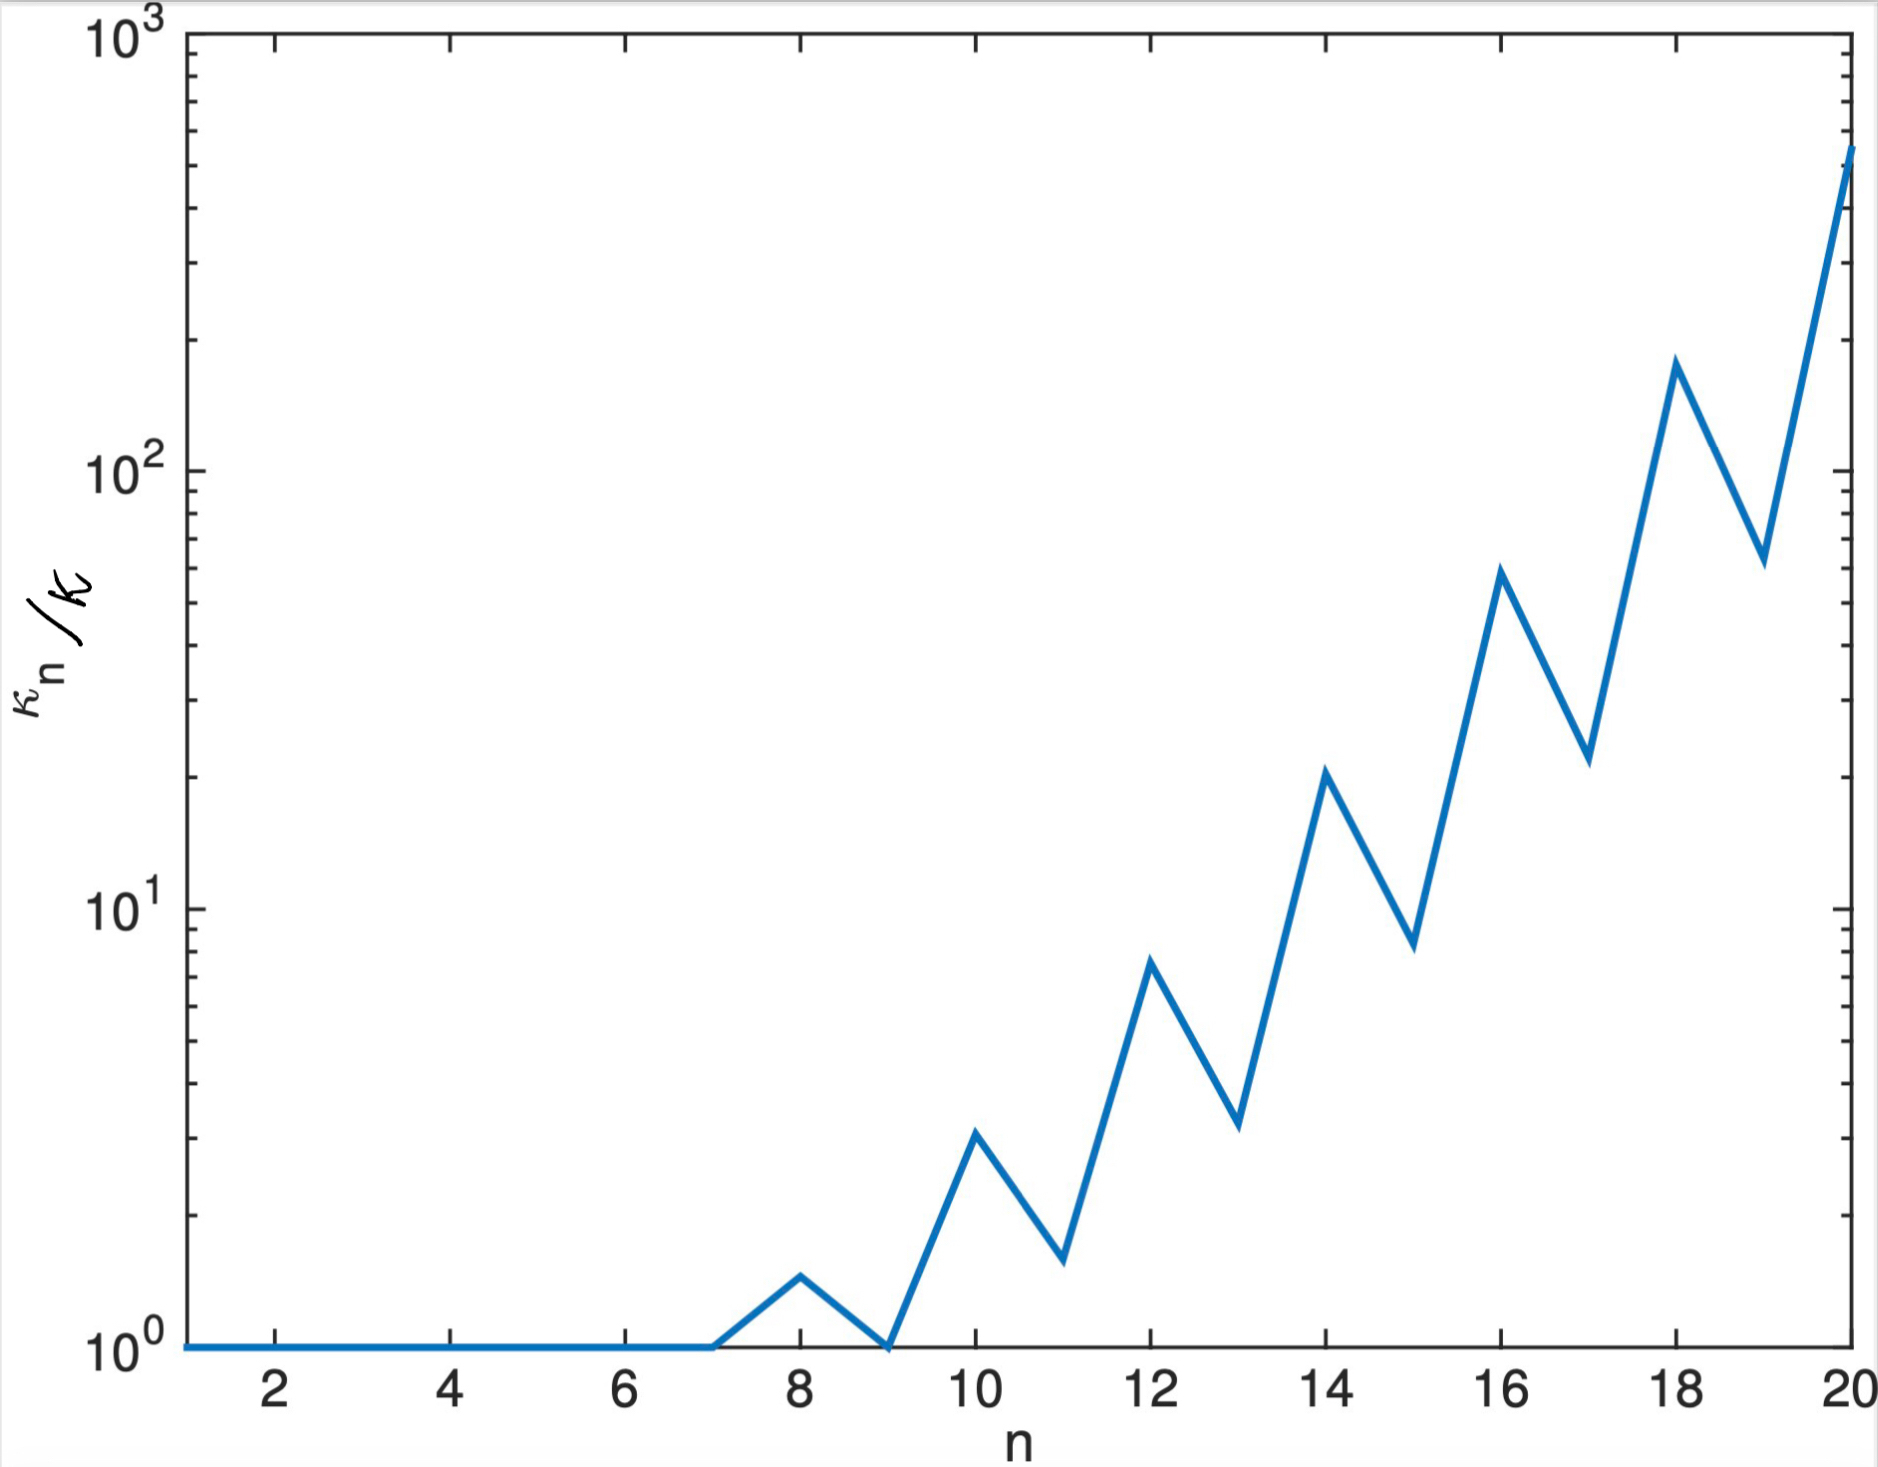
\includegraphics[width=0.5\textwidth]{immagini/knN-C.png}
    \caption{numero di condizionamento (\ref{eq:nrCondN-C}) delle formule di Newton-Cotes nel caso $b-a=1$.}\label{fig:knN-C}
\end{figure}

\subsection{Errore (di quadratura) e formule composite}
\subsubsection{Errore di quadratura}
\footnote{Slide 8 PDF 26 PG 108.} Discutere l'accuratezza di $I_n(f)$ significa quantificare l'errore di quadratura
\begin{equation}\label{eq:errQuadr}
    \begin{matrix}
        \boldsymbol{E_n(f)}&\boldsymbol{\equiv}& I(f)-\overset{\footnotemark}{I_n(f)}&=&\int_a^b f(x)dx-\int_a^bp_n(x)dx\\
        &=&\int_a^b\underbrace{(f(x)-p_n(x))}_{\footnotemark}dx&=&\int_a^bf[x_0,\hdots,x_n,x]\omega_{n+1}(x)dx\\
        &&\int_a^bf[x_0,\hdots,x_n,x]\prod_{i=0}^n(x-x_i)dx&\overset{\footnotemark}{=}&\boldsymbol{\nu_n} \underbrace{\boldsymbol{f^{(n+\mu)}(\xi)}}_{\footnotemark}\boldsymbol{\left(\frac{b-a}{n}\right)^{n+\mu+1}},\quad\xi\in [a,b],
    \end{matrix}
\end{equation}
\addtocounter{footnote}{-3}
\footnotetext{È esattamente l'integrale del polinomio interpolante la $f$.}

\stepcounter{footnote}
\footnotetext{Errore di interpolazione.}

\stepcounter{footnote}
\footnotetext{L'errore ha una struttura che nel caso $n$ sia dispari è facile da dimostrare, non è così per $n$ pari.}

\stepcounter{footnote}
\footnotetext{Assunto che $f\in C^{(n+\mu)}[a,b]$.}
\noindent dove:
\begin{itemize}
    \item $\boldsymbol{\nu_n}$ è una costante che dipende solo da $n$ (ed è limitata uniformemente);
    \item $\boldsymbol{\mu}=
    \begin{cases}
        \boldsymbol 1, &\text{se $n$ è dispari;}\\
        \boldsymbol 2, &\text{se $n$ è pari.}
    \end{cases}$
\end{itemize}

Se $n$ è dispari, è calcolata la derivata $n+1$ (dove 1 è $\mu$). Quindi la formula è esatta se è un polinomio di grado $n$, quando $n$ è dispari. Questo fatto è noto perché il polinomio di grado $n$ interpolante la funzione, la quale è un polinomio di grado $n$, coincide con la funzione stessa.

Se $n$ è pari, l'intergrale è esatto per i polinomi di grado $n+1$ e la derivata $f^{(n+\mu)}(\xi)$, con $m=2\rightarrow n+2$, si annulla se $f$ è un polinomio di grado $n+1$.

Quanto appena descritto è l'osservazione seguente.

\begin{remark}
    \footnote{Slide 10 PDF 26, Corollario 5.1 PG 110.} Una formula di Newton-Cotes di grado $n$, calcolata su $n+1$ punti, è esatta per integrandi polinomiali fino al grado:
    \begin{equation*}
        \begin{cases}
            n, &\text{se $n$ dispari};\\
            n+1, &\text{se $n$ pari}.
        \end{cases}
    \end{equation*}
\end{remark}

Dato $E_n(f)$ in forma (\ref{eq:errQuadr}) non è possibile affermare che $\left(\frac{b-a}{n}\right)^{n+\mu +1}\rightarrow 0,$ per $ n\rightarrow\infty$, a causa del condizionamento del problema. Per risolvere questo problema è necessario decrementare il rapporto $\frac{b-a}{n}$ senza fare crescere $n$, utilizzando un approccio simile a quello delle spline nel caso di interpolazione, ovvero: l'intervallo $[a,b]$ è suddiviso in più sottointervalli di uguale ampiezza ed è utilizzata, su ciascun intervallo, la formula di Newton-Cotes di grado $k$ fissato. Così facendo sono ottenute le formule di Newton-Cotes composite.
\footnote{L'idea è la seguente: date le ascisse è applicato su ciascun sottointervallo una formula di grado $k$ fissato. Con il numero di questi sottointervalli che tende all'infinito allora, la formula di grado $k$ viene applicata su intervalli sempre più piccoli. Ciò significa che il termine $\frac{b-a}{n}$ si trasformerà in $\left(\frac{b-a}{k}\right)^n$, dove $k$ è il grado della formula ed $n$ il numero di punti.}

\subsubsection{Formula dei trapezi composita}
\begin{definition}[\textbf{Formula dei trapezi composita}]\footnote{Slide 11 PDF 26.}
    Siano $\{x_i\}$ ascisse equidistanziate definite come in (\ref{eq:condAscEqN-C}), è ottenuta la \textbf{formula dei trapezi composita}:
    \begin{equation}\label{eq:formTrapComp}
        \begin{matrix}
            \boldsymbol{I(f)}&=&\int_a^b f(x) dx &\overset{\footnotemark}{=}&\sum_{i=1}^n\overbrace{\int_{x_{i-1}}^{x_i} f(x)dx}^{\footnotemark}\\
            &\approx& h\sum_{i=2}^n\frac{f(x_{i-1})+f(x_i)}{2} &\boldsymbol\equiv& \boldsymbol{I_1^{(n)}(f)}\\
            &=& h\left(\frac{f_0}{2}+\frac{f_1}{2}+\frac{f_1}{2}+\hdots +\frac{f_{n-1}}{2}+\frac{f_{n-1}}{2}+\frac{f_n}{2}\right)&\boldsymbol =&\boldsymbol{h\left(\frac{f_0}{2}+\sum_{i=1}^{n-1}f_i+\frac{f_n}{2}\right)}
        \end{matrix}
    \end{equation}
\end{definition}

\addtocounter{footnote}{-1}
\footnotetext{L'intervallo è diviso in sottointervalli e quindi l'area totale è la somma delle aree parziali, le quali sono approssimate con le funzioni trapezi.}

\stepcounter{footnote}
\footnotetext{Ogni integrale è una parte dell'area del sottografo.}

\begin{remark}
    \footnote{Slide 12 PDF 25.} Se $f(x)$ è periodica allora $f_n=f_0\Rightarrow I_1^{(n)}(f)=h\underset{\footnotemark}{\sum_{i=0}^{n-1}f_i}.$ 
\end{remark}\footnotetext{La complesità del calcolo della sommatoria è $\log (n)$ perché sommando 2 a 2 i risultati sommati 2 a 2 è possibile arrivare ad un'approssimazione in $\log (n)$ passi. Se la funzione è periodica allora è possibile approssimarla con $\sin$ e $\cos$, per le quali l'approssimazione diviene esatta, per polinomi parametrici di grado sempre più elevato, man mano che cresce $n$. Ciò significa che è possibile ottenere delle approssimazioni molto accurate di un segnale periodico (con $\sin$ e $\cos$).}

\begin{definition}[\textbf{Errore di quadratura formula dei trapezi}]
    L'\textbf{errore commesso} dalla \textbf{formula dei trapezi} è il seguente:
    \begin{equation}\label{eq:errFormTrapComp}
        \begin{matrix}
            E_1^{(n)}(f) &\overset{\footnotemark}{=}& I(f)-I_1^{(n)}(f)\\
            &\overset{\footnotemark}{=}&\nu_1 \left(\frac{b-a}{n}\right)^3 \sum_{i=1}^n f^{(2)}(\xi_i),\quad \xi_i\in[x_{i-1},x_i]\\
            &=& \nu_1 \left(\frac{b-a}{\boldsymbol n}\right)^{\boldsymbol 3}\boldsymbol n  f^{(2)}(\xi),\quad \xi\in[a,b] \\
            &=& \nu_1 \boldsymbol{(b-a)}f^{(2)}(\xi)\,\boldsymbol{\left(\frac{b-a}{n}\right)^2}\rightarrow 0,\; n\rightarrow\infty.
        \end{matrix}
    \end{equation}
\end{definition}

\addtocounter{footnote}{-1}
\footnotetext{Somma di $\sum_{i=1}^n \int_{x_{i-1}}^{x_i} f(x)dx$ e $h\sum_{i=2}^n\frac{f(x_{i-1})+f(x_i)}{2}$.}

\stepcounter{footnote}
\footnotetext{Come in seguito, vale il teorema della sommazione discreta, ovvero: data la derivata seconda continua $f^{(2)}$ (successiva all'uguale nella sommatoria) e sommando $n$ valori che appartengono ad $n$ sottointervalli contigui allora $f^{(2)}$ sarà uguale ad $n$ volte il valore della derivata seconda in un parametro dell'intervallo. Inoltre, $\nu_1=-\frac{1}{12}$, cosa non specificata a lezione. La scelta di $\nu_1$ viene fatta risolvendo un sistema di equazioni che impone che l'errore di quadratura sia nullo per funzioni polinomiali di grado $0$ e $1$. In questo caso, è possibile arrivare alla conclusione che $\nu_1=-\frac{1}{12}$ è la scelta giusta per garantire la convergenza di ordine $O\left((b-a)^3\right)$.}

\begin{remark}
    La formula dei trapezi composita può essere implementata come nell'Algoritmo \ref{alg:trapec}.
\end{remark}

\subsubsection{Formula di Simpson composita}
\begin{definition}[\textbf{Formula di Simpson composita}]
    Siano $\{x_i\}$ ascisse equidistanziate definite come in (\ref{eq:condAscEqN-C}) e dato $\boldsymbol n$ \textbf{pari}, la \textbf{formula di Simpson composita} è
    \begin{equation}\label{eq:formSimpComp}
        \begin{matrix}
            \boldsymbol{I(f)}&=&\int_a^bf(x)dx\\
            &=&\sum_{i=1}^{\frac{n}{2}}\int_{x_{2(i-1)}}^{x_{2i}}f(x)dx\\
            &\overset{\footnotemark}{\approx}&\frac{b-a}{3\cdot n}\sum_{i=1}^{\frac{n}{2}}(f(x_{2(i-1)})+4f(x_{2i-1})+f(x_{2i}))\\
            &\underset{\footnotemark}{=}&\frac{b-a}{3n}(\underline{f_0+4f_1+f_2}+\underline{f_2+4f_3+f_4}+\hdots+\underline{f_{n-2}+4f_{n-1}+f_n})\\
            &=&\frac{b-a}{3n}\underbrace{\left[4\sum_{i=1}^{\frac{n}{2}}f_{2i-1}+2\sum_{i=0}^{\frac{n}{2}}f_{2i}-f_0-f_n\right]}_{\footnotemark}&\boldsymbol\equiv& \boldsymbol{I_2^{(n)}(f)}.
        \end{matrix}
    \end{equation}
\end{definition}

\addtocounter{footnote}{-2}
\footnotetext{Approssimazione che necessita di 3 ascisse, ovvero da $x_0$ a $x_1$, da $x_2$ a $x_4$ e così via, dove l'ascissa in mezzo è quella pesata con 4.}

\stepcounter{footnote}
\footnotetext{4 è associato ai numeri con indice dispari ($f_1,\, f_3,\hdots,\, f_{n-1})$. Gli elementi con indice pari, tranne il primo e l'ultimo, hanno coefficiente 2 perché appartenenti a due intervalli congiunti.}

\stepcounter{footnote}
\footnotetext{Quando le sommatorie dovranno essere implementate in Matlab sarà necessario sfruttare le capacità di calcolo vettoriale di Matlab. Non sono necessari cicli ma è possibile calcolare una valutazione vettoriale della $f$ su tutte le ascisse per poi pesare le componenti in modo opportuno. Sarà visto un esempio nelle esercitazioni.}

\begin{definition}[\textbf{Errore di quadratura formula di Simpson}]
    L'\textbf{errore commesso} dalla \textbf{formula di Simpson} è il seguente:
    \begin{equation}\label{eq:errFormSimpComp}
        E_2^{(n)}(f)=I(f)-I_2^{(n)}(f)=\nu_2 f^{(4)}(\xi)\left(\frac{b-a}{n}\right)^5 = \nu_2f^{(4)}(\xi)\frac{b-a}{2}\left(\frac{b-a}{n}\right)^{\overset{\footnotemark}{4}}\rightarrow 0,\; n\rightarrow\infty,\quad \xi\in[a,b],
    \end{equation}
    dove $\nu_2 = -\frac{1}{180}$ (cosa non speficiata a lezione).
    \footnotetext{$\frac{n}{2}=\frac{2}{2}+\mu=2+1$, con $n$ numero di termini.}
\end{definition}

Questa procedura si generalizza per tutte le formule di Newton-Cotes di grado $k$, a patto che $n$ sia un multiplo di $k$, ottenendo la formula di Newton-Cotes di grado $k$ è espressa come
\begin{equation*}
    I_k^{(n)}=h\sum_{i=0}^nf_ic_{ik}=h\sum_{i=0}^nf_i\int_0^k\prod_{j=0, j\neq i}^k\frac{t-j}{i-j},
\end{equation*}
e l'errore associato come
\begin{equation}\label{eq:EkComposite}
 E_k^{(n)}(f)=\nu_kf^{(k+\mu)}(\xi)\frac{b-a}{k}\left(\frac{b-a}{n}\right)^{k+\mu}, \quad \xi\in[a,b],
\end{equation}
dove $E_k^{(n)}(f)\rightarrow 0,\, n\rightarrow\infty$.

\paragraph{Spiegazione notazione $\boldsymbol{E_k^{(n)}(f)}$:} $k$ è il grado della formula base, $n$ sono i punti utilizzati sui quali è applicata la formula di quadratura composita. Ciò significa che per far diminuire l'errore è possibile far aumentare $n$ lasciando $k$ fisso.

\begin{example}
    Come esempio, esplicato tramite la Figura \ref{fig:approxIntSinx}, è approssimato tramite la formula composita dei trapezi e con quella di Simpson il seguente integrale:
    \begin{equation}\label{eq:approxIntSinx}
        \int_0^\pi \sin{x}dx\quad (=2).
    \end{equation}
    Dalla Figura \ref{fig:approxIntSinx} è possibile notare che l'approssimazione di Simpson sia migliore di quella dei trapezi perché più precisa.
\end{example}

\begin{figure}
    \centering
    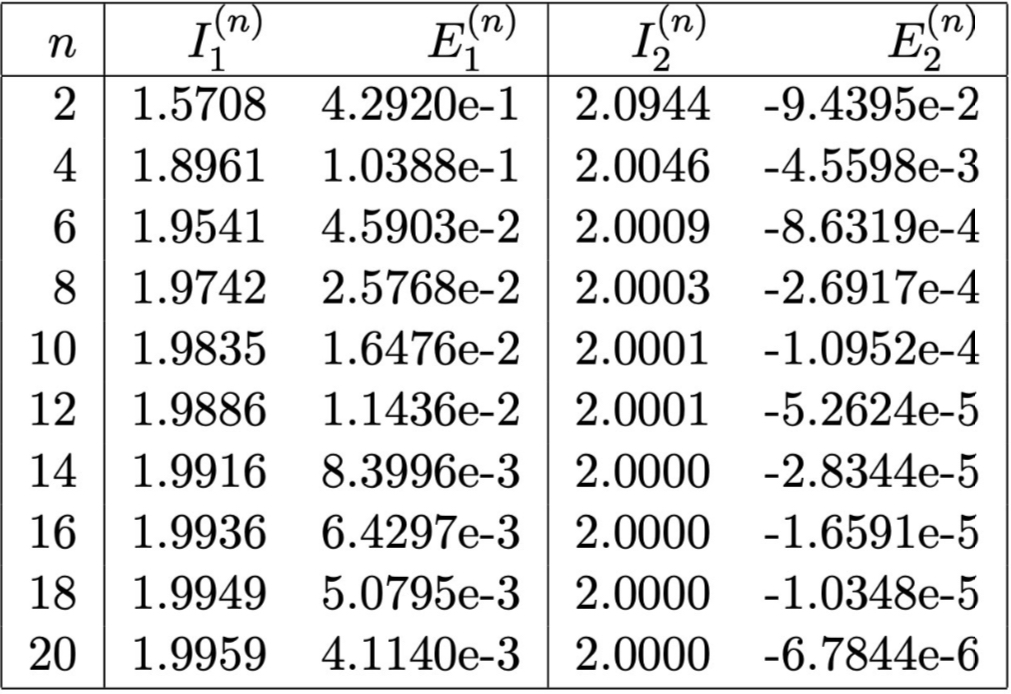
\includegraphics[width=0.5\textwidth]{immagini/approxIntSinx.png}
    \caption{Approssimazione e corrispondenti errori di (\ref{eq:approxIntSinx}).}\label{fig:approxIntSinx}
\end{figure}

L'espressione (\ref{eq:EkComposite}) permette di derivare, \textbf{a costo nullo} (cosa importante), una stima dell'errore di quadratura, $E_k^{(n)}(f)$, nel caso in cui $\boldsymbol n$ \textbf{sia un multiplo pari di} $\boldsymbol k$.

È necessario che $n$ sia un multiplo di $k$, affinché lo sia anche $\frac{n}{2}$, cosicché sia possibile valutare $\boldsymbol{I_k^{(\frac{n}{2})}(f)}$. $\boldsymbol{I_k^{(\frac{n}{2})}(f)}$ è calcolato su ascisse di indice pari ($0,2,4,\hdots$) e la valutazione di $I_k^{(\frac{n}{2}}(f)$ è ottenuta senza ulteriori valutazioni della funzione $f(x)$ perché è possibile utilizzare le valutazioni
\begin{equation*}
    \boldsymbol{f_{2i}\equiv f(x_{2i}),\quad i=0,\hdots,\frac{n}{2}},
\end{equation*}
le quali sono già calcolate per la valutazione di $I_k^{(n)}(f)$. \footnote{Sono calcolate le valutazioni funzionali di $f$ per calcolare $I_n^k(f)$ e utilizzate quelle con indice pari così da calcolare $I_n^k$. Il costo della formula di quadratura è maggiorato in un numero di valutazioni di funzioni con costo nullo.} Pertanto, analogamente a (\ref{eq:errFormSimpComp}), vale:
\begin{equation}\label{eq:errFormSimpCompN/2}
    I(f)-I_k^{(\frac{n}{2})}(f)=\nu_k f^{(n+\mu)}(\into{\widehat\xi}{[a,b]})\frac{b-a}{k}\left(\frac{b-a}{n/2}\right)^{n+\mu}\overset{\footnotemark}{\approx}\nu_k f^{(n+\mu)}(\xi)\frac{b-a}{k}\left(\frac{b-a}{n}\right)^{n+\mu}2^{n+\mu}.
\end{equation}\footnotetext{Fingendo che $\widehat\xi=\xi$ e trasformando $\frac{n}{2}$ in $2^{n+\mu}$ allora è possibile l'approssimazione.}

Sottraendo membro a membro (\ref{eq:EkComposite}) a (\ref{eq:errFormSimpCompN/2}) allora:
\begin{equation*}
    I_k^{(n)}(f)-I_k^{(\frac{n}{2})}\approx\boldsymbol{\nu_kf^{(n+\mu)}(\xi)\frac{b-a}{k}\left(\frac{b-a}{n}\right)^{n+\mu}}(2^{n+\mu}-1)\equiv \left(\boldsymbol{I(f)-I_k^{(n)}(f)}\right)(2^{n+\mu}-1).
\end{equation*}

In altri termini, è possibile ottenere una stima dell'errore di quadratura $E_k^{(n)}(f)$ come:
\begin{equation*}
    \boldsymbol{E_k^{(n)}(f)\approx\frac{I_k^{(n)}(f)-I_k^{(\frac{n}{2})}(f)}{2^{n+\mu}-1}\equiv\widehat E_k^{(n)}(f)}.
\end{equation*}

Applicando quanto scritto all'esempio (\ref{eq:approxIntSinx}) sono derivate le Figure \ref{fig:approxInt}-\ref{fig:tabErrQuad}.

\begin{figure}
    \centering
    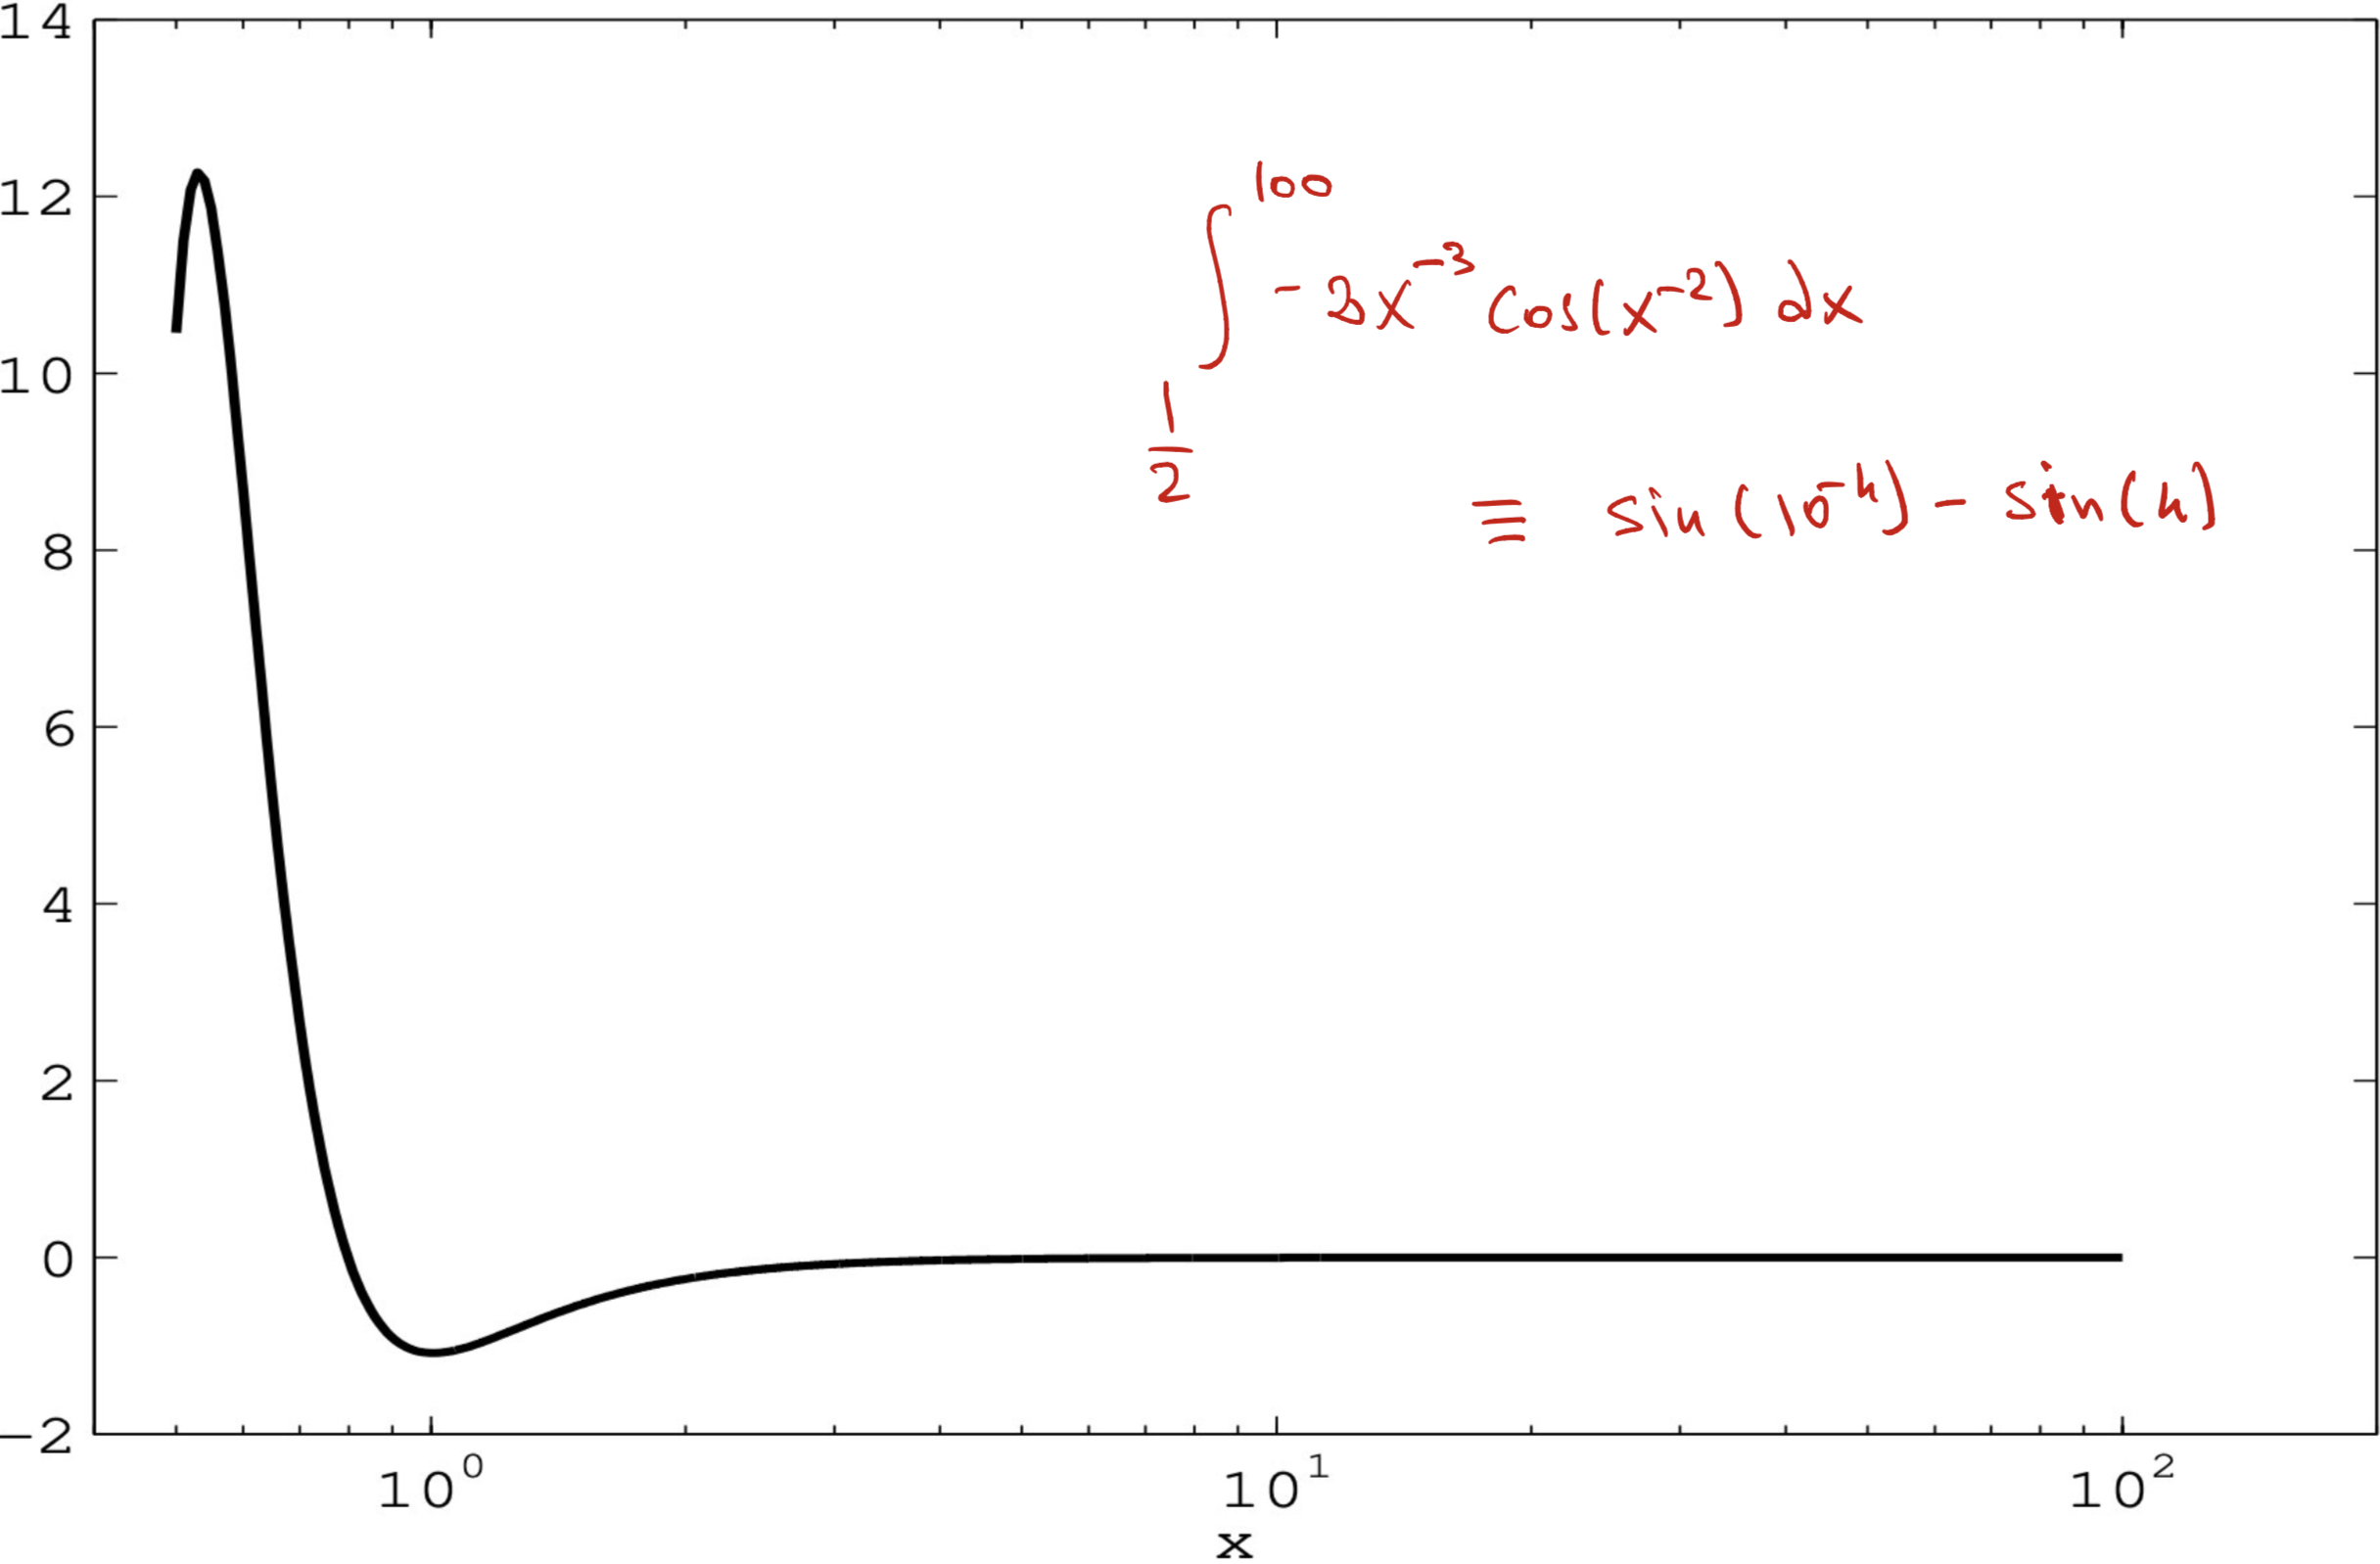
\includegraphics[width=0.5\textwidth]{immagini/approxInt.jpg}
    \caption{Approssimazione $\int_{\frac{1}{2}}^{100}-2x^{-3}\cos(x^{-2})$.}\label{fig:approxInt}
\end{figure}

\begin{figure}
    \centering
    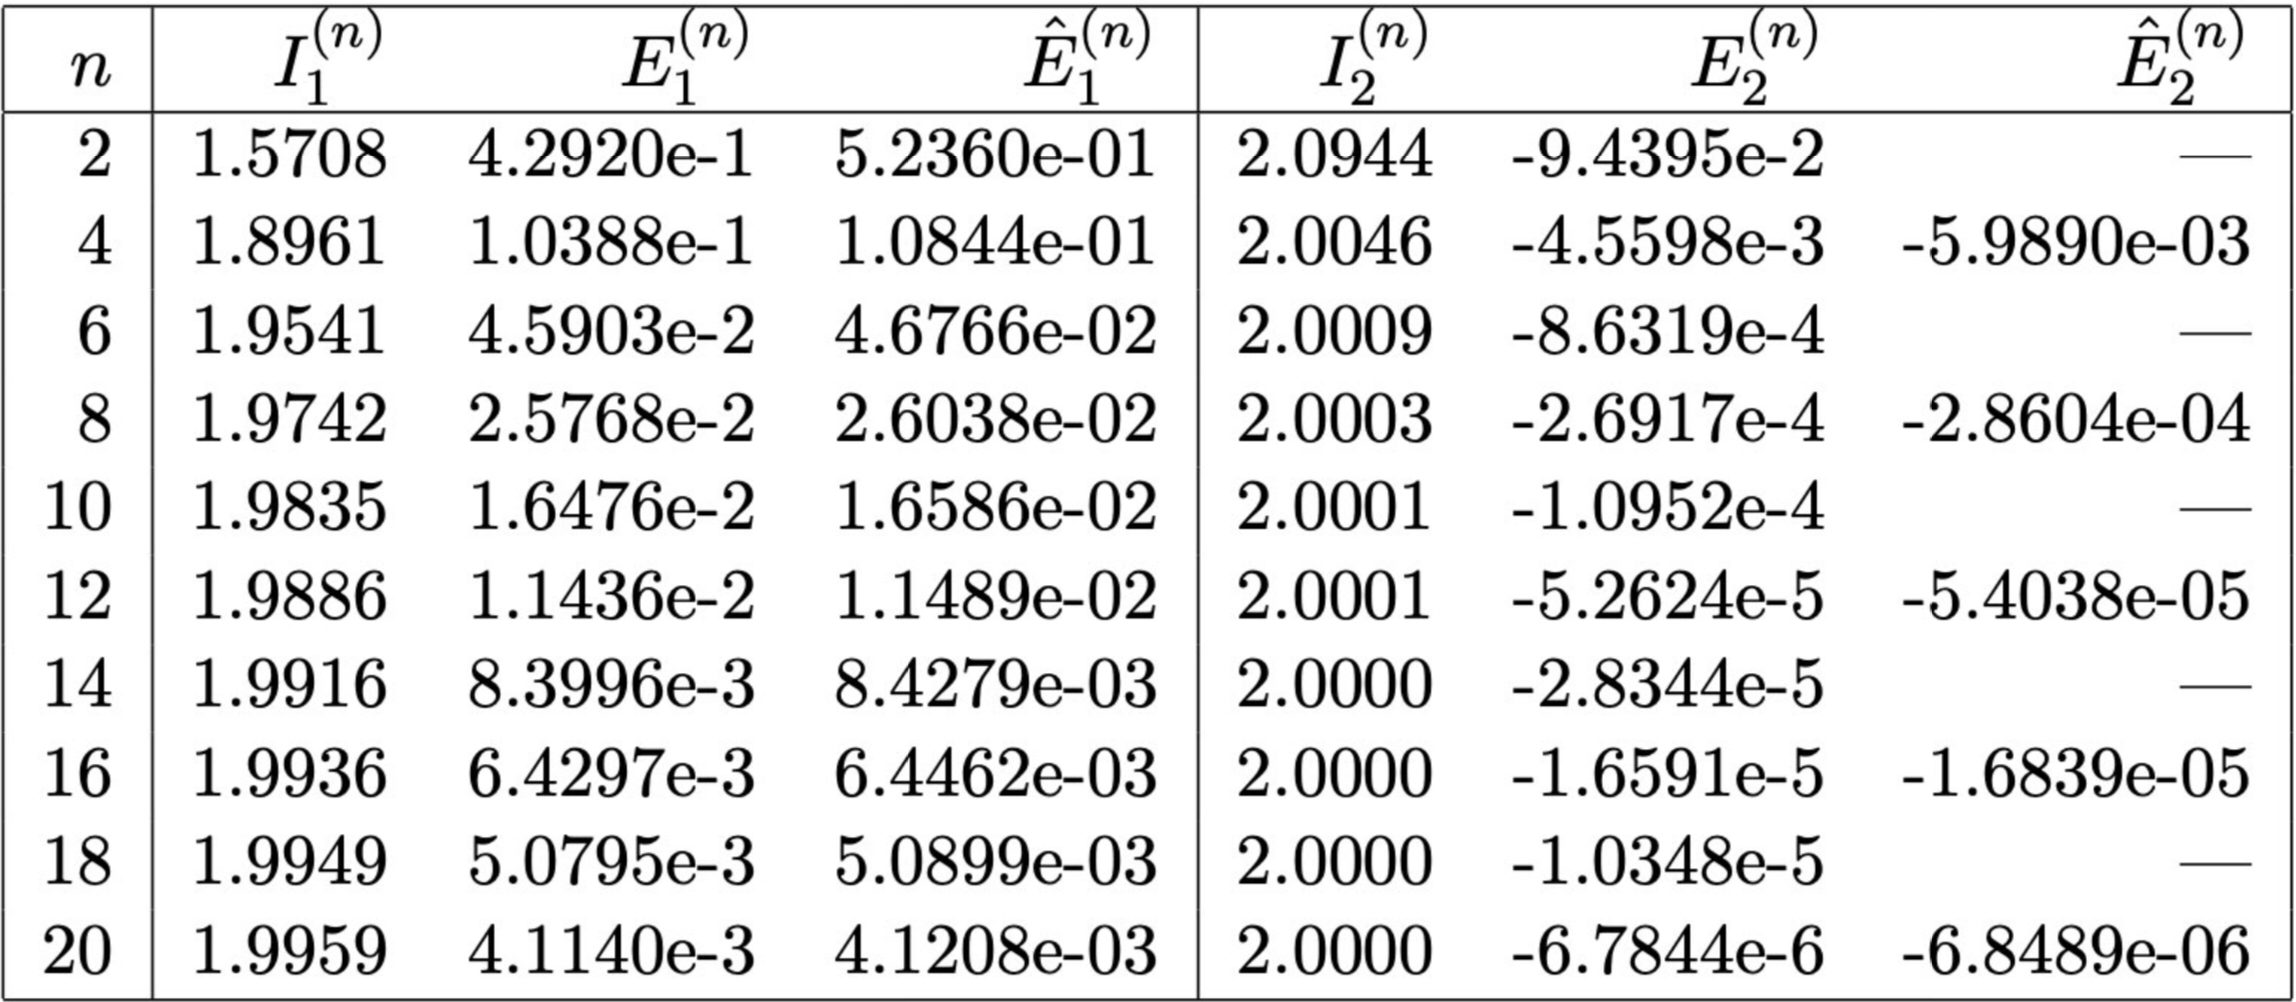
\includegraphics[width=0.5\textwidth]{immagini/tabErrQuad.png}
    \caption{Confronto fra errore di quadratura approssimazione con formula di quadratura dei trapezi e di Simpson.}\label{fig:tabErrQuad}
\end{figure}

In Figura \ref{fig:approxInt} il numero di condizionamento è 99.5, ovvero l'ampiezza dell'intervallo. Il problema è che nell'estremo inferiore, se $x\rightarrow 0$, allora $x^{-2}$ e $x^{-3}$ diventano molto grandi e $\cos{(x^{-2})}$, per $x\rightarrow 0$, oscilla molto. La parte sinistra del grafico è la parte in cui il grafico inizia ad oscillare molto. La questione importante è che la funzione è liscia poco dopo $10^0$ e oscilla poco prima di $10^0$. Se fosse utilizzata una mesh costante accadrebbe che, per ottenere la tolleranza desiderata, diventerebbero necessari punti molto vicini prima di $10^0$, i quali dovrebbero essere riportati anche nella parte liscia. Il problema posto è quello di definire un approccio adattivo per la definizione delle ascisse di interpolazione in modo adattivo, infatti sui punti laddove la funzione è più variabile saranno inseriti più punti ed invece meno dove la funzione è liscia. Per quanto appena scritto, sono introdotte le funzioni di Newton-Cotes adattive della Sezione \ref{ssec:formN-CAdatt}.
In Figura \ref{fig:tabErrQuad} è possibile notare che tanto più cresce $n$ più l'errore diminuisce e quindi aumenta la precisione. È necessario trattare il fatto che, nell'implementazione di queste formule, le ascisse sono tutte equidistanti. Le ascisse equidistanti sono definite come (\ref{eq:condAscEqN-C}).

\subsection{Formule di Newton-Cotes adattive}\label{ssec:formN-CAdatt}
\footnote{Slide 7-12 PDF 27, PG 111-114.}
Il problema è trovare un metodo per definire le ascisse in base al comportamento della funzione. Dal punto di vista algoritmico è interessante ciò che sarà visto nell'implementazione dei casi più semplici, ovvero dei trapezi e di Simpson, con Matlab, tramite function ricorsive. In ogni caso è sfruttato il fatto he esiste un'espressione asintotica dell'errore quadratico.

\subsubsection{Formula dei trapezi}
In questo caso, con $n=1$, è ottenuto (da (\ref{eq:errQuadr}))
\begin{equation}\label{eq:errQuadN=1}
    I(f)-I_1(f)=\nu_1 f^{(2)}(\xi)(b-a)^3\quad \xi\in[a,b],
\end{equation}
ed è ottenuto che, da (\ref{eq:errFormTrapComp}), applicando la formula composita su due sottointervalli ($n=2$), ciò che segue:\begin{equation}\label{eq:errQuadN=2}
    I(f)-I_1^{(2)}(f)=\nu_1 f^{(2)}(\xi)(b-a)\left(\frac{b-a}{2}\right)^2,\quad \xi\in [a,b],
\end{equation}
dove $\nu_1=-\frac{1}{12}$

Suppondendo che gli $\xi$ di (\ref{eq:errQuadN=2}) da (\ref{eq:errQuadN=1}) siano simili, sottraendo (\ref{eq:errQuadN=2}) da (\ref{eq:errQuadN=1}) è ottenuto che
\begin{equation*}
    \boldsymbol{I_1^{(2)}(f)-I_1(f)}\approx\nu_1 f^{(2)}(\xi)(b-a)\left(\frac{b-a}{2}\right)^2\underset{\footnotemark}{(4-1)}\equiv \left(\boldsymbol{I(f)-I_1^{(2)}(f)}\right) 3
\end{equation*}
allora
\begin{equation*}
    \boldsymbol{E_1^{(2)}(f)\equiv I(f)-I_1^{(2)}(f)\approx\frac{I_1^{(2)}(f)-I_1(f)}{3}}.
\end{equation*}

\footnotetext{Dovuto a $\left(\frac{b-a}{2}\right)^2$ in (\ref{eq:errQuadN=2}) ed a $(b-a)^3$ in (\ref{eq:errQuadN=1}).}

La procedura adattiva è generata con il prossimo passo: Supponendo di dover calcolare $I(f)$ con una accuratezza $\boldsymbol{tol}$ (parametro prefissato, ovvero scelto dall'utente), se $\left|E_1^{(2)}\leq tol\right|$ è terminata la procedura, altrimenti è riapplicata la stessa procedura sui due sottointervalli $\left[a,\frac{a+b}{2}\right],\, \left[\frac{a+b}{2},b\right]$, con tolleranza $\boldsymbol{tol/2}$.

In questo modo è definito, in modo adattivo, l'insieme dei punti su quali sono applicate le formule base e la sua composita raddoppiata.

Quindi il passo di raffinamento esplicito funziona nel seguente modo: se è soddisfatta l'accuratezza richiesta la procedura si ferma, altrimenti il problema è diviso in 2 sottoproblemi, ai quali è applicato separatamente la stessa procedura con tolleranza dimezzata. Il dimezzamento è applicato affinché la somma degli errori sia sempre piccola. Se questa procedura è applicata ricorsivamente laddove l'errore è maggiore allora questo sarà affinato maggiormente, mentre qualora l'errore soddisfa il requisito di accuratezza la procedura si ferma. Questa procedura definisce adattivamente le ascisse, sulle quali sono definite le formule di quadratura.

\subsubsection{Formula di Simpson}
Similmente, per la formula di Simpson ($n=2$ su $[a,b]$), è ottenuto che:
\begin{equation}\label{eq:stimaErrFormQuadSimpN=2}
    I(f)-I_2(f)=\nu_2 f^{(4)}(\xi)\left(\frac{b-a}{2}\right)^{\overset{\footnotemark}{5}},\quad \xi\in[a,b].
\end{equation}
\footnotetext{$\mu=1$ perché $k$ è pari.}

Se è applicata la formula di Simpson composita con $n=4$ su $[a,b]$, è ottenuto:
\begin{equation}\label{eq:stimaErrFormQuadSimpCompN=4}
    I(f)-I_2^{(4)}(f)=\nu_2 f^{(4)}(\widehat\xi)\frac{b-a}{2}\left(\frac{b-a}{4}\right)^4,\quad \widehat\xi\in[a,b],
\end{equation}
dove in (\ref{eq:stimaErrFormQuadSimpN=2}) e (\ref{eq:stimaErrFormQuadSimpCompN=4}) $\nu_2=-\frac{1}{90}$.

Con $\widehat\xi\approx\xi$ (\ref{eq:stimaErrFormQuadSimpN=2}) diviene
\begin{equation}\label{eq:trasfXiToXi}
    I(f)-I_2(f)\approx\nu_2 f^{(4)}(\widehat\xi)\frac{b-a}{2}\left(\frac{b-a}{4}\right)^4\cdot 16.
\end{equation}

Sottraendo (\ref{eq:trasfXiToXi}) da (\ref{eq:stimaErrFormQuadSimpCompN=4}) è ottenuto
\begin{equation*}
    I_2^{(4)}(f)-I_2(f)\approx\nu_2 f^{(4)}(\widehat\xi)\frac{b-a}{2}\left(\frac{b-a}{4}\right)^4(16-1)\equiv E_2^{(4)}(f)\cdot 15.
\end{equation*}
Da questo risultato è ottenuto che l'errore di quadratura $E_2^{(4)}(f)$ può essere stimato come
\begin{equation}
    \boldsymbol{E_2^{(4)}(f)\approx\underbrace{\frac{I_2^{(4)}(f)-I_2(f)}{15}}_{\text{Numero}}}.
\end{equation}

\footnote{È importante notare, sarà fatto nell'esercitazione, che quando sono replicate le procedure, in modo ricorsivo, come vengono riciclate le valutazioni già calcolate, passandole come parametro, al fine di costruire l'albero ricorsivo.}
Pertanto, è richiesta un'accuratezza $\boldsymbol{tol}$ per il calcolo di $I(f)$: se $\left|E_2^{(4)}(f)\right|\leq tol$ la procedura si arresta, altrimenti riapplicando stessa procedura sui due sottointervalli $\left[a,\frac{a+b}{2}\right]$ e $\left[\frac{a+b}{2},b\right]$, con tolleranza $\boldsymbol{tol/2}$.

Ciò che è importante è notare che il procedimento è adattivo ed automatico. La formula dei trapezi è quella meno accurata. La formula di Simpson ha un ordine di accuratezza che è il quadrato di quello dei trapezi.
Inoltre, osservando $E_1^{(n)}$ e $E_2^{(n)}$ è possibile notare che $E_1^{(n)}$ è quasi il quadrato di $E_2^{(n)}$. Questo deriva dal fatto che $\mu=2$, per la formula di Simpson e $\mu=1$ per la formula dei trapezi.

\begin{remark}
    \footnote{Slide 10 PDF 27.} help \textbf{integral}.
\end{remark}

\begin{figure}
    \centering
    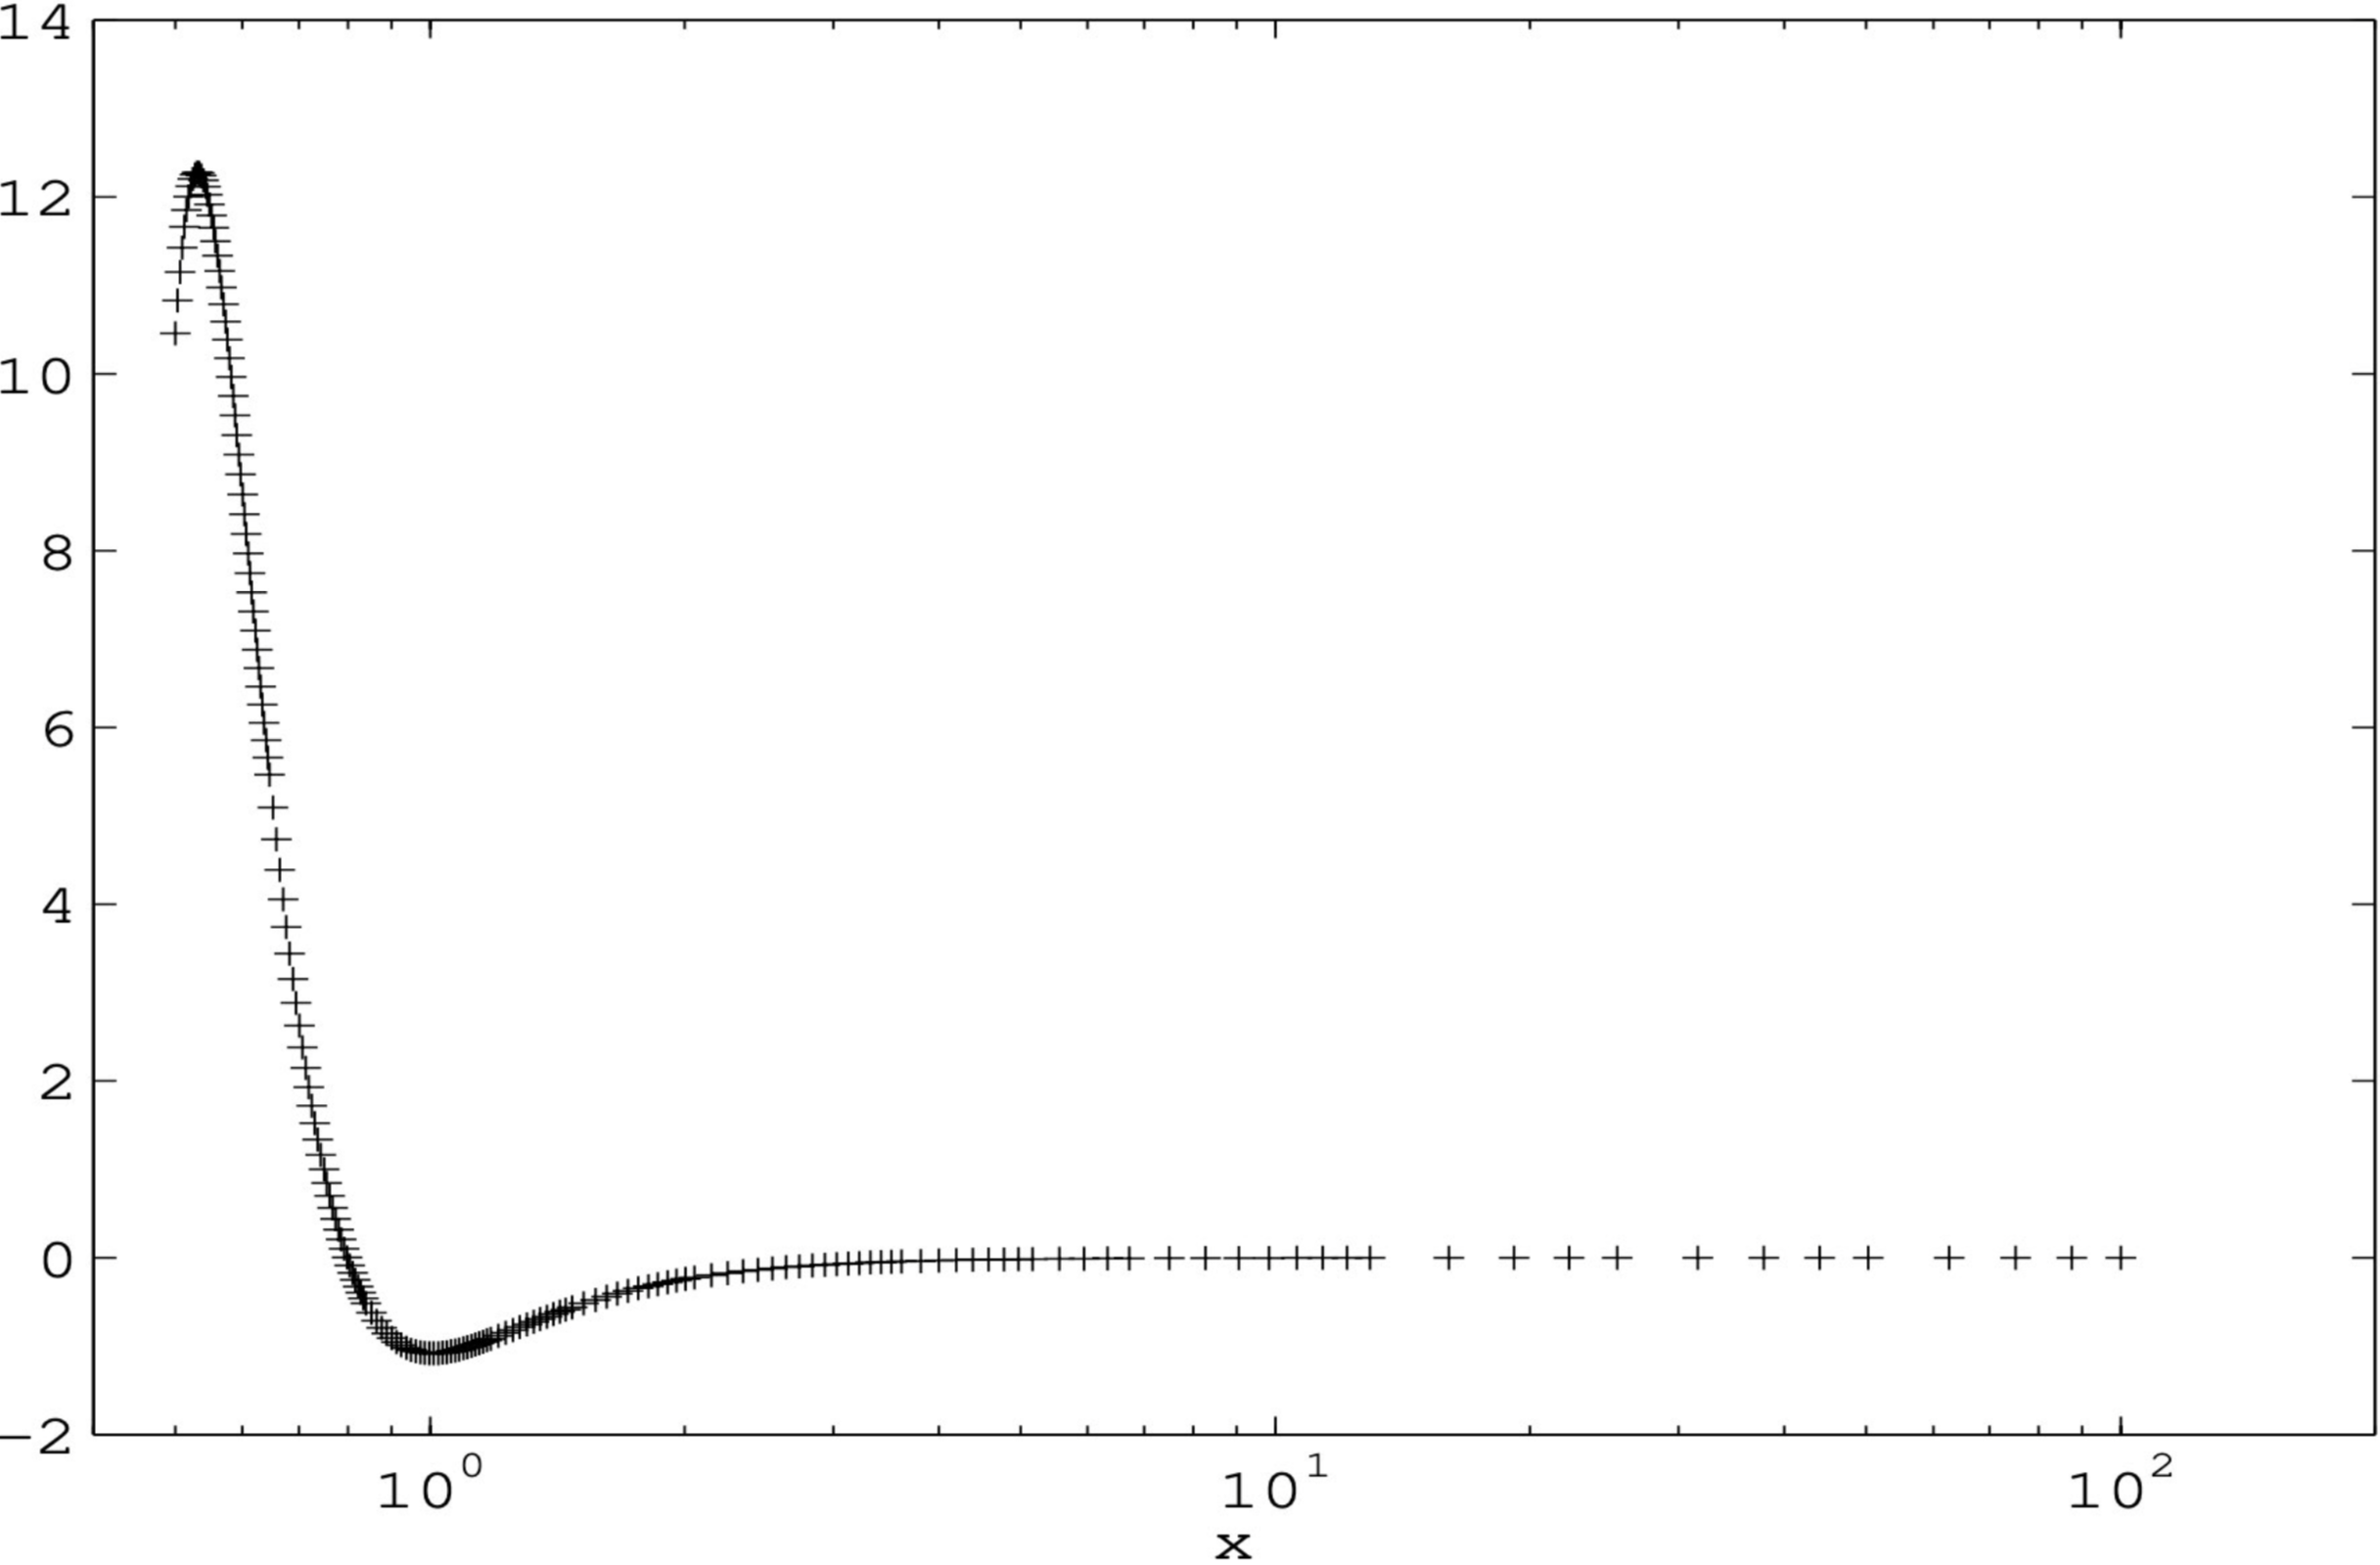
\includegraphics[width=0.5\textwidth]{immagini/simpsonAdatToll=10e-5.png}
    \caption{Simpson adattivo con $\boldsymbol{tol=10e-5}$.}\label{fig:simpsonAdatToll=10e-5}
\end{figure}

\begin{algorithm}\caption{Implementazione algoritmo adattivo dei trapezi.}
\label{alg:algAdattFormTrap}
    \begin{lstlisting}[style=Matlab-editor]
    function I2 = adaptrap(f, a, b, tol, fa, fb)
    %
    % Utilizzo:tab I2 = adaptrap(f, a, b, tol) [questa e' un'interfaccia utente, viene invocata la prima volta. fa e fb sono utilizzati per implementare la funzione ricorsivamente, quindi dalla seconda invocazione della function] [Nel caso della function che implementa la funzione Simpson e' necessario prevere 3 valutazioni funzionali, non come nelle implementazioni della formula dei trapezi, la quale richiede due valutazioni in input]
    %
    % Input:
    %   f - function handler funzione integranda;
    %   a,b - estremi intervallo di integrazione;
    %   tol - accuratezza richiesta.
    %
    % Output:
    %   I2 - approssimazione ottenuta.
    if nargin < 4 
        error('numero argomenti insufficienti')
    end
    if tol <= 0 
        error('tolleranza nulla o minore di 0')
    end 
    if nargin == 4
        fa = feval(f, a); fb = feval(f, b);
    end
    h = b - a;
    x1 = (a + b)/2;
    f1 = feval(f, x1); %valutazione funzionale nel punto medio
    I1 = (h/2)*(fa+fb); 
    I2 = (I1 + h*f1)/2; 
    e = abs(I2-I1)/3; %stima dell'errore
    if e > tol
        I2 = adaptrap(f, a, x1, tol/2, fa, f1)...
            + adaptrap(f, x1, b, tol/2, f1, fb); 
    end
    return
    \end{lstlisting}
\end{algorithm}
